%!TEX root = notas_de_clase.tex

\newpage
\centerline{--------------------------------- clase X/4/18 ---------------------------------}
\section{Selección de Modelo}
Supongamos que tenemos un montón de datos, de los cuales podemos ajustar un millón de modelos, tanto como la imaginación nos limite. Entonces ¿Con cuál te quedarías al final?
Cuando nos enfrentamos a la decisión de elegir un modelo usualmente lo que más interesa es la preciso del modelo a la hora de generalizar. El problema de solo buscar precisión es claro: \emph{overfitting} (ver figura \ref{fig:overfitting}).
\begin{figure}[h!]
    \centering
    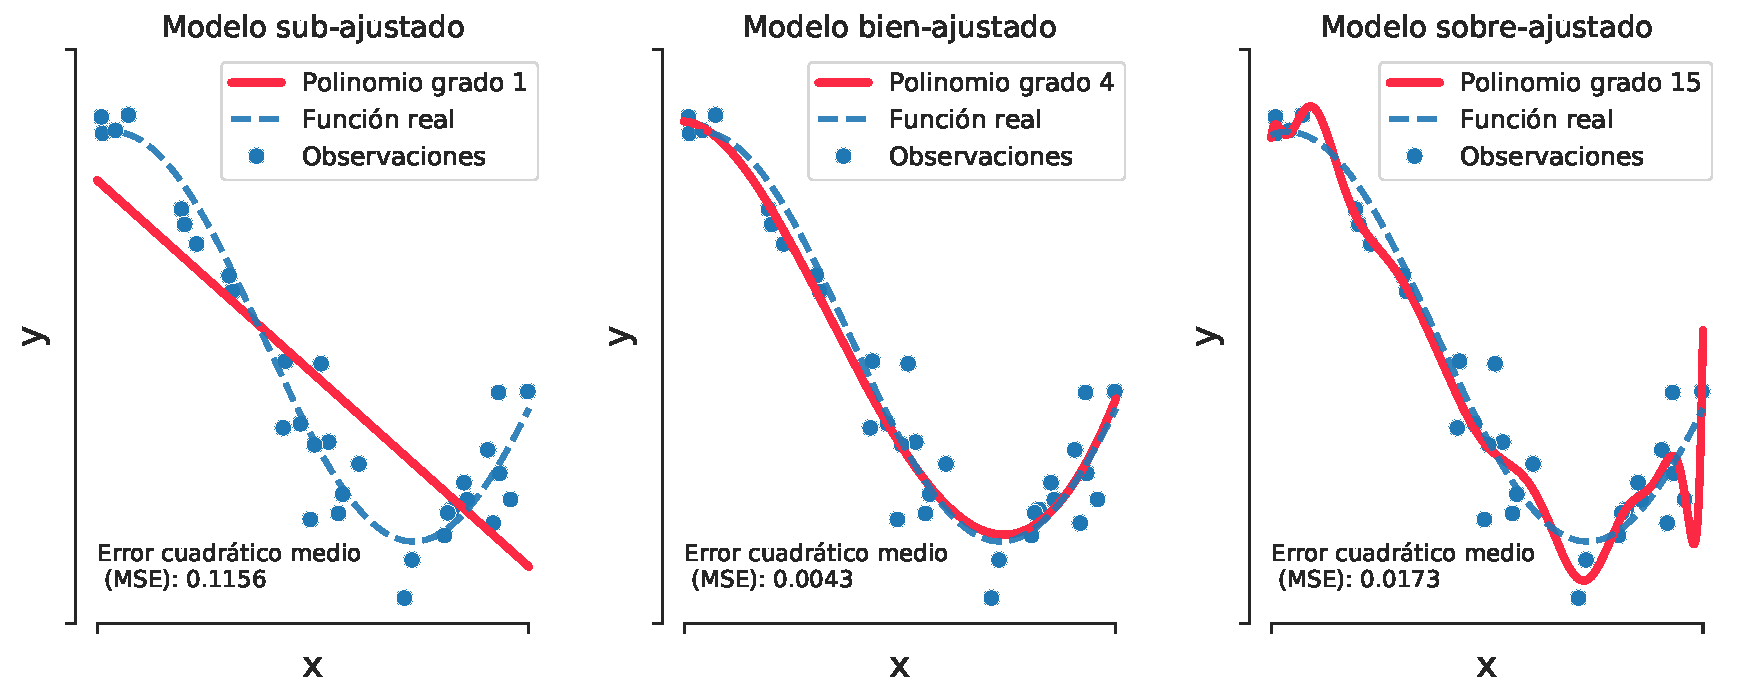
\includegraphics[width = 0.9\linewidth]{img/cap3_ajuste.pdf}
    \caption{Ejemplos de sub, sobre y correcto ajuste.}
    \label{fig:overfitting}
\end{figure}

La elección de modelo es uno de los problemas más recurrentes en análisis de datos, un ejemplo es la elección de las variables para la regresión ¿Por qué elegir un modelo cuadrático y no uno cúbico? ¿Por qué no incorporar todas las variables cruzadas ($X_1X_2, X_1X_3, ..., X_nX_m$)? Estas preguntas son fácilmente abordables si volvemos a la realidad y queremos correr los modelos en nuestros computadores: Incorporar más variables usualmente aumenta la complejidad computacional y con esto el tiempo de cómputo.

Bajo la filosofía anterior, encontrar un  \textit{trade-off} entre \emph{bias} (la flexibilidad del modelo de ajustarse a los datos) y performance sería lo ideal. Es por esta razón que crear un estadístico que pudiera expresar correctamente el compromiso precisión - flexibilidad ayudaría en la elección de modelo. Esto último es lo que busca relizar el \emph{Akaike Information Criterion} (AIC) y el \emph{Bayesian Information Criterion} (BIC) los cuales son dos enfoques distintos para abordar esta problemática.

\subsection{Criterio de Información Akaike}
La siguiente aproximación es válida cuando $N \to \infty$:

\begin{equation*}
-2\mathbb{E}[\log P_{\hat{\theta}}(Y)] \approx \frac{-2}{N}\mathbb{E}[\log L] + 2\frac{d}{N},
\end{equation*}

en donde $d$ es la cantidad de parámetros del modelo y  $L$ es la función de verosimilitud definida por:

\begin{equation}
L = \prod_{i=1}^N P(y_i|\hat{\theta}).
\end{equation}

De esta manera se define el estadístico AIC de la forma:

\begin{equation}
AIC(M) = 2d-2\log(L)
\end{equation}

Otros autores definen el estadístico como:

\begin{equation}
AIC(M) = 2\frac{d}{N}-2\frac{log(L)}{N}.
\end{equation}
Donde N es la cantidad de observaciones.

\textbf{\underline{Ejemplo:}} Si tenemos un conjunto de modelos $f_{\alpha}(x)$ indexados por un parámetro $\alpha$ de modo que el modelo $\alpha$ sigue un modelo gaussiano, es decir:
$$
\log(L) = -\sum_{i}(y_i-\hat{f}(x_i))^2/(2\sigma_e^2),
$$

\noindent entonces el estimador AIC se puede escribir como
\begin{equation}
\text{AIC}(M) = 2d(\alpha)-\overline{err}(\alpha),
\end{equation}
en donde la función $d(\alpha)$ denota una medida de la complejidad del modelo y $\overline{err}(\alpha)$ denota el error promedio del modelo $\alpha$.

\subsection{Criterio de Información Bayesiano}
Nuevamente, si nuestro setting nos permite obtener el máximo de la función de verosimilitud. Podemos utilizar el \emph{Bayesian Information Criterion} (BIC) el cual está definido por:

\begin{equation}
\text{BIC}(M) = log(N)d-2\log(L)
\end{equation}

En donde N es la cantidad de observaciones, $d$ es la cantidad de parámetros del modelo y L es el máximo de la función de verosimilitud. Este criterio también es conocido como \emph{Schwarz criterion}. Este estadístico se dice bayesiano por que se obtiene de realizar una aproximación de laplace sobre sobre $\log\mathbb{P}(X|M)$ obteniéndose:

\begin{equation}
\log\mathbb{P}(X|M) \approx \log\mathbb{P}(X|\hat{\theta}_m, M) - \frac{d_m}{2}(\log(N)-\log(2\pi))
\end{equation}

Donde $\hat{\theta}_m$ es el máximo del estimador de verosimilitud. Luego para $N$ muy grande se observa que la expresión $-2\log\mathbb{P}(X|M) = BIC(M)$.

\textbf{\underline{Ejemplo:}} Asumiendo que el modelo sigue un modelo gaussiano, es decir:
$$
\log(L) = -\sum_{i}(y_i-\hat{f}(x_i))^2/(2\sigma_e^2),
$$se tiene que el estadístico BIC está dado por:

\begin{equation}
BIC(M) = \frac{N\overline{err}(M)}{\sigma_e^2} + log(N)d
\end{equation}


\subsection{Evaluación y comparación de modelos}
Existen varias formas de evaluar un modelo, una de ella podría ser simplemente evaluar la precisión de sus predicciones. A veces fijarse es natural fijarse en la precisión, como en los problemas de pronóstico. Otras veces la precisión es importante para evaluar diferentes modelos y elegir uno de ellos. En esta sección presentaremos dos maneras distintas de evaluar modelos, cada forma sirve en distintos escenarios, los cuales se discutirán a través de la predicción puntal, que resume la predicción de un conjunto de datos en una solo valor.

\subsubsection{Error cuadrático medio}

El ajuste del modelo a nuevos datos se puede resumir en una predicción puntual llamada error cuadrático medio, el cual está definido por:

\begin{equation}
MSE(\theta) = \frac{1}{n}\sum_{i=1}^N (y_i-\mathbb{E}(y_i|\theta))^2
\end{equation}

o su versión ponderada:

\begin{equation}
MSE(\theta) = \frac{1}{n}\sum_{i=1}^N \frac{(y_i-\mathbb{E}(y_i|\theta))^2}{\mathbb{V}\text{ar}(y_i|\theta)}
\end{equation}

\subsubsection{log-densidad predictiva o log-verosimilitud}
Otra forma de realizar esta evaluación es utilizando el estadístico \emph{log-densidad preditiva} $\log p(y|\theta)$ el cual es proporcional a error cuadrático medio si el modelo es normal con varianza constante. Estudiaremos el caso de un solo punto, para luego extrapolar a más de un punto.

\textbf{Predictive accuracy para un punto}: Sea $f$ el modelo real, $y$ las observaciones (es decir, una realización del dataset $y$ de la distribución $f(y)$), y llamaremos $\tilde{y}$ a la data futura o un dataset alternativos que podemos ver. El ajuste predictivo out-of-sample para un nuevo punto $\tilde{y}_i$ está dado por:

\begin{equation}
\log p_{\text{post}}(\tilde{y}_i) = \log \mathbb{E}[p(\tilde{y}_i|\theta)] = \log \int p(\tilde{y}_i|\theta)p_{\text{post}}(\theta)d\theta
\end{equation}

\textbf{Promedio de las distribuciones para un punto}: Al tener un dato nuevo $\tilde{y}_i$ entonces se puede calcular el la log-densidad predictiva (elpd, por su sigla en inglés) para el nuevo punto:
\begin{align}
\notag \text{elpd} & = \mathbb{E}_f[\log p_{\text{post}}(\tilde{y}_i)]\\
& = \int \log p_{\text{post}}(\tilde{y}_i) f(\tilde{y}_i)d\tilde{y}
\end{align}

\textbf{Promedio de las distribuciones para datasets futuros}: Como usualmente, no se tiene solo un punto, se debe realizar la suma sobre el conjunto de puntos, calculando así la log-densidad predicitiva puntual (elppd, por su sigla en inglés).

\begin{align}
\text{elppd} & = \sum_{i=1}^N \mathbb{E}_f[\log p_{\text{post}}(\tilde{y}_i)]
\end{align}

En la práctica, como siempre se tiene la distribución de todos los modelos y la expresión anterior requiere de esto, se suele calcular el estadístico sobre una estimación de un modelo $\hat{\theta}$ (como por ejemplo, el máximo de la función de verosimilitud):

\begin{align}
\text{elppd}|\hat{\theta} & = \sum_{i=1}^N \mathbb{E}_f[\log p_{\text{post}}(\tilde{y}_i|\hat{\theta})]
\end{align}

Finalmente, una última extensión de este estadístico es cuando se puede tener \emph{draws} de la posterior, es decir, tenemos $\{ \theta^s\}_{s=1}^S$, entonces el lppd computado es:

\begin{equation}
\text{computed lppd} = \sum_{i=1}^N \left( \frac{1}{S} \sum_{s=1}^S p(y_i|\theta^s)\right)
\end{equation}

\subsubsection{Otros métodos}
Existen otros estadísticos o métodos que se pueden utilizar para comparar modelos. 

\begin{itemize}
    \item \textbf{Deviance Information Criterion:} Se podría decir que es una versión bayesiana de AIC, donde se realizan dos cambios principales 1) se cambia la estimación del estimador de máxima verosimilitud, por el promedio de la posterior y 2) se reemplaza k con una perrción de sesgo de los datos. Formalizando:
    
    \begin{equation}
        \text{DIC} = -2 \log(y|\hat{\theta}_{Bayes}) + 2p_{\text{DIC}},
    \end{equation}
    donde $p_{\text{DIC}}$ está dado por:
    
    \begin{equation}
        p_{\text{DIC}} = 2(\log(p(y|\hat{\theta}_{Bayes})- \mathbb{E}_{\text{post}}(\log(p(y|\theta)).
    \end{equation}
    
    Nuevamente, puede haber un versión \emph{computada} que está dada por:
    
    \begin{equation}
        \text{computed }p_{\text{DIC}} = 2[\log(p(y|\hat{\theta}_{Bayes})- \frac{1}{S}\sum_{s=1}^S \log (p(y|\theta^s))].
    \end{equation}
    %-------------------------------
    \item \textbf{Watanabe-Akaike o widely available information criterion:} WAIC es un forma aún más bayesiana para abordar el problema de asginación de evaluación. 
    
    \begin{equation}
        \text{WAIC} = -2 \text{lppd} + 2 p_{\text{WAIC}}
    \end{equation}
    
    donde hay dos formas de calcular $p_{\text{WAIC}}$.
    
    \begin{align}
    p_{\text{WAIC}1} &= 2 \sum_{i= 1}^n \left( \log(\mathbb{E}_{\text{post}}[p(y_i|\theta)]) - \mathbb{E}_{\text{post}}[\log (p(y_i|\theta))\right)\\
    p_{\text{WAIC}2} &= \sum_{i= 1}^n \left( \mathbb{V}\text{ar}_{\text{post}}[\log(p(y_i|\theta))]\right).
    \end{align}
    %-------------------------------    
    \item \textbf{Leave-one-out cross-validation:} También se puede usar validación cruzada bayesiana para estimar $-2\text{lppd} + 2\text{lppd}_{\text{loo-cv}}$ la cual sirve como estadístico de comparación:
    
    \begin{equation}
    \text{lppd}_{\text{loo-cv}} = \sum_{i=1}^n \log p_{\text{post}(-i)}(y_i)
    \end{equation}
    
    que se calcula como:
    
    \begin{equation}
    \text{computed lppd}_{\text{loo-cv}} = \sum_{i=1}^n \log \left( \sum_{s=1}^S \frac{1}{S} p(y_i|\theta^{is})\right)
    \end{equation}
    
    también se puede calcular a versión insesgada, la cual no se utiliza mucho pero se presenta por completitud:
    \begin{equation}
    \text{lppd}_{\text{cloo-cv}} = \text{lppd}_{\text{loo-cv}} + b.
    \end{equation}
    Donde $b$ está dado por:
    
    \begin{align}
    b = \text{lppd}_{-i} - \overline{\text{lppd}_{-i}},
    \end{align}
    
    con 
    
    \begin{align}
    \overline{\text{lppd}_{-i}} & = \frac{1}{n} \sum_{i=1}^n\sum_{j=1}^n \log p_{\text{post}(-i)}(y_j)\\
    \text{computed }\overline{\text{lppd}_{-i}} & = \frac{1}{n} \sum_{i=1}^n\sum_{j=1}^n \log \left( \frac{1}{S}\sum_{s=1}^S p(y_j|\theta^{is})\right).
    \end{align}
    
\end{itemize}

\subsection{Promedio de Modelos}
Hay veces que no queremos elegir solo un modelo, puesto que quizás nos interesan las estimaciones de dos o más modelos. Para estos casos, se puede utilizar la técnica de \emph{Model Averaging}, la cual consiste en simplemente ponderar los modelos de la siguiente forma:

\begin{equation}
\hat{\mu} = \sum_{s\in A} c(s) \hat{\mu}_s
\end{equation}
donde $A$ es el conjunto de todos los modelos. Además, se debe cumplir que:
\begin{equation}
\sum_{s\in A} c(s) = 1
\end{equation}

Notemos que la elección:

\begin{equation}
c(s) =
\begin{cases}
1 & \text{modelo con mejor criterio.}\\
0 & \sim
\end{cases}
\end{equation}

es una elección de pesos posible.

\subsubsection{Elección de pesos mediante softmax}

La principal dificultad para elegir los pesos, está en que se debe asegurar 1) la suma de los pesos sea unitaria, 2) que los pesos sean todos positivos. Una forma de asegurar esto es aplicar una función $f$ positiva sobre una función $g$ de \emph{score}, de modo que:

\begin{equation}
\sum_{s\in A} (f\circ g)(s) > 0
\end{equation}

Así los pesos quedan se pueden definir cómo:

\begin{equation}
c_f(s) = \frac{(f\circ g)(s)}{\sum_{z\in A} (f\circ g)(s)}
\end{equation}

La elección más común de para $f(x) = \text{softmax}(x)$, mientras que para la función de \emph{score} se puede utilizar las recién estudiadas AIC o BIC.

\begin{align}
c_{AIC}(s) = \frac{\exp\{ \frac{1}{2} \text{AIC}_s\}}{\sum_{z\in A} \exp\{ \frac{1}{2} \text{AIC}_z\}} & & c_{BIC}(s) = \frac{\exp\{ \frac{1}{2} \text{BIC}_s\}}{\sum_{z\in A} \exp\{ \frac{1}{2} \text{BIC}_z\}}
\end{align}


\subsubsection{Bayesian Model Averaring}

Supongamos que tenemos $\{M_j\}_{j=1}^k$ modelos, de los cuales todos realizan estimaciones razonables de una cantidad $\mu$, dado los datos $y$.
Para realizar el modelo promedio bayesiano de estos modelos es necesario encontrar la distribución posterior de $\mu$ dado los datos $y$ sin condicionar a un modelo en específico. De este modo, es necesari:
\begin{enumerate}
    \item Cada modelo tenga los mismos puntos de interpolación.
    \item Prior para cada modelo $p(M_j)$.
    \item Prior sobre los parámetros de los modelos $\pi(\theta_i|M_j)$\footnote{Se puede obtener mediante MCMC.}.
\end{enumerate}


Luego se puede calcular la función de verosimilitud para los parámetros:

\begin{equation}
\mathcal{L}_{\theta_j}(y) = p(y|\theta_j)
\end{equation}

Luego se marginaliza sobre los parámetros para obtener la función de verosimilitud del modelo:

\begin{align}
\lambda_{M_j}(y) & = p(y|M_j)\\
& = \int \mathcal{L}_{\theta_j}(y) \pi(\theta_i|M_j) d\theta_j\label{eq:lambda}
\end{align}

La expresión \eqref{eq:lambda} es también densidad marginal de las observaciones. Con esto la densidad posterior del modelo es:

\begin{align}
p(M_j|y) = \frac{p(M_j)\lambda_{M_j}(y)}{\sum_{l=1}^k p(M_{l})\lambda_{M_{l}}(y)}    
\end{align}

Finalmente, se puede obtener la distribución posterior para $\mu$ asumiendo que el modelo $M_j$ es verdadero ($\pi(\mu|M_j,y)$), y así, la distribución posterior buscada:

\begin{equation}
\pi(\mu|y) = \sum_{j = 1}^k p(M_j|y)\pi(\mu|M_j,y)
\end{equation}

